\documentclass[14pt, a4 paper]{report}
\usepackage{graphicx} % Required for inserting images
\usepackage{caption}
\usepackage{subcaption}
\usepackage{listings}
\usepackage{amsmath}

\usepackage[utf8]{inputenc}
\usepackage[T1]{fontenc}
\DeclareMathSymbol{\invques}{\mathord}{operators}{`>}
\DeclareUnicodeCharacter{00BF}{\tmquestiondown}
\DeclareRobustCommand{\tmquestiondown}{%
  \ifmmode\invques\else\textquestiondown\fi
}
\usepackage[portuges]{babel}%Babel -- irá activar automaticamente as regras apropriadas de hifenização para a língua todo o
                                   %-- o texto gerado é automaticamente traduzido para Português.
                                   %  Por exemplo, “chapter” irá passar a “capítulo”, “table of contents” a “conteúdo”.
                                   % portuges -- específica para o Português.
\usepackage[utf8]{inputenc} % define o encoding usado texto fonte (input)--usual "utf8" ou "latin1
\usepackage{parcolumns}

\usepackage{graphicx} %permite incluir graficos, tabelas, figuras
\usepackage{url} % para utilizar o comando \url{}
\usepackage{enumerate} %permite escolher, nas listas enumeradas, se os iems sao marcados com letras ou numeros-romanos em vez de numeracao normal

%\usepackage{apalike} % gerar biliografia no estilo 'named' (apalike)

\usepackage{color} % Para escrever em cores
\usepackage{multirow} %tabelas com multilinhas
\usepackage{array} %formatação especial de tabelas em array
\usepackage[pdftex]{hyperref} % transformar as referências internas do seu documento em hiper-ligações.
\usepackage{listings}
\usepackage{xcolor}
\definecolor{codegreen}{rgb}{0,0.6,0}
\definecolor{codegray}{rgb}{0.5,0.5,0.5}
\definecolor{codepurple}{rgb}{0.58,0,0.82}
\definecolor{backcolour}{rgb}{0.95,0.95,0.92}

\lstdefinestyle{mystyle}{
    backgroundcolor=\color{backcolour},   
    commentstyle=\color{codegreen},
    keywordstyle=\color{magenta},
    numberstyle=\tiny\color{codegray},
    stringstyle=\color{codepurple},
    basicstyle=\ttfamily\footnotesize,
    breakatwhitespace=false,         
    breaklines=true,                 
    captionpos=b,                    
    keepspaces=true,                 
    numbers=left,                    
    numbersep=5pt,                  
    showspaces=false,                
    showstringspaces=false,
    showtabs=false,                  
    tabsize=2
}

\lstset{style=mystyle}

%Exemplos de fontes -- nao e vulgar mudar o tipo de fonte
%\usepackage{tgbonum} % Fonte de letra: TEX Gyre Bonum
%\usepackage{lmodern} % Fonte de letra: Latin Modern Sans Serif
%\usepackage{helvet}  % Fonte de letra: Helvetica
%\usepackage{charter} % Fonte de letra:Charter

\definecolor{saddlebrown}{rgb}{0.55, 0.27, 0.07} % para definir uma nova cor, neste caso 'saddlebrown'

\usepackage{listings}  % para utilizar blocos de texto verbatim no estilo 'listings'
%paramerização mais vulgar dos blocos LISTING - GENERAL
\lstset{
	basicstyle=\small, %o tamanho das fontes que são usadas para o código
	numbers=left, % onde colocar a numeração da linha
	numberstyle=\tiny, %o tamanho das fontes que são usadas para a numeração da linha
	numbersep=5pt, %distancia entre a numeração da linha e o codigo
	breaklines=true, %define quebra automática de linha
    frame=tB,  % caixa a volta do codigo
	mathescape=true, %habilita o modo matemático
	escapeinside={(*@}{@*)} % se escrever isto  aceita tudo o que esta dentro das marcas e nao altera
}
%
%\lstset{ %
%	language=Java,							% choose the language of the code
%	basicstyle=\ttfamily\footnotesize,		% the size of the fonts that are used for the code
%	keywordstyle=\bfseries,					% set the keyword style
%	%numbers=left,							% where to put the line-numbers
%	numberstyle=\scriptsize,				% the size of the fonts that are used for the line-numbers
%	stepnumber=2,							% the step between two line-numbers. If it's 1 each line
%											% will be numbered
%	numbersep=5pt,							% how far the line-numbers are from the code
%	backgroundcolor=\color{white},			% choose the background color. You must add \usepackage{color}
%	showspaces=false,						% show spaces adding particular underscores
%	showstringspaces=false,					% underline spaces within strings
%	showtabs=false,							% show tabs within strings adding particular underscores
%	frame=none,								% adds a frame around the code
%	%abovecaptionskip=-.8em,
%	%belowcaptionskip=.7em,
%	tabsize=2,								% sets default tabsize to 2 spaces
%	captionpos=b,							% sets the caption-position to bottom
%	breaklines=true,						% sets automatic line breaking
%	breakatwhitespace=false,				% sets if automatic breaks should only happen at whitespace
%	title=\lstname,							% show the filename of files included with \lstinputlisting;
%											% also try caption instead of title
%	escapeinside={\%*}{*)},					% if you want to add a comment within your code
%	morekeywords={*,...}					% if you want to add more keywords to the set
%}

\usepackage{xspace} % deteta se a seguir a palavra tem uma palavra ou um sinal de pontuaçao se tiver uma palavra da espaço, se for um sinal de pontuaçao nao da espaço

\parindent=2pt %espaço a deixar para fazer a  indentação da primeira linha após um parágrafo
\parskip=4pt % espaço entre o parágrafo e o texto anterior

\setlength{\oddsidemargin}{-1cm} %espaço entre o texto e a margem
\setlength{\textwidth}{18cm} %Comprimento do texto na pagina
\setlength{\headsep}{-1cm} %espaço entre o texto e o cabeçalho
\setlength{\textheight}{23cm} %altura do texto na pagina

% comando '\def' usado para definir abreviatura (macros)
% o primeiro argumento é o nome do novo comando e o segundo entre chavetas é o texto original, ou sequência de controle, para que expande
\def\darius{\textsf{Darius}\xspace}
\def\antlr{\texttt{AnTLR}\xspace}
\def\VM{\href{https://ewvm.epl.di.uminho.pt/}{VM}}
\def\plc{\emph{Processamento de Linguagens e Compiladores}\xspace}
\def\titulo#1{\section{#1}}    %no corpo do documento usa-se na forma '\titulo{MEU TITULO}'
\def\super#1{{\em Supervisor: #1}\\ }
\def\area#1{{\em \'{A}rea: #1}\\[0.2cm]}
\def\resumo{\underline{Resumo}:\\ }
\def\e#1{\emph{#1}}

%\input{LPgeneralDefintions} %permite ler de um ficheiro de texto externo mais definições

\title{Computação Gráfica (3º ano de LCC)\\
       \textbf{Trabalho Prático (Fase 3) — Grupo 3}\\ Relatório de Desenvolvimento}
\author{André Lucena Ribas Ferreira (A94956) 
    \and Carlos Eduardo da Silva Machado (A96936)
    \and Gonçalo Manuel Maia de Sousa (A97485)}
\date{\today} %data

\begin{document}

\maketitle

\begin{abstract}
    Este relatório aborda a solução proposta para o enunciado da 3ª fase do Trabalho Prático da Unidade Curricular "Computação Gráfica". 
\end{abstract}

\tableofcontents

\chapter{Introdução} \label{chap:intro}

O presente relatório tem como objetivo apresentar a solução concebida pelo Grupo 3 para a 2ª fase do Trabalho Prático da Unidade Curricular "Computação Gráfica". 

Esta fase consistiu na atualização da forma como os modelos são desenhados para utilizar as vantagens dos \textbf{VBOs}. Como escolha do grupo, decidimos que o iríamos fazer utilizando índices cuidadosamente escolhidos para usufruir de vantagens de localidade espacial. Também era necessário implementar variações para as transformações de rotação e de translação, através do tempo de rotação e de curvas de Catmull-Rom. Por fim, foi necessário dotar o \textit{generator} da capacidade de ler ficheiros \textit{batch} que, com uma dada estrutura, descrevem superfícies de Bezier, para poder construir primitivas gráficas a partir dessas superfícies. 

À demo desta parte, foi acrescentado o movimento de translação e rotação de cada planeta e do Sol tal como um modelo a partir destas superfícies que representa um cometa a viajar pelo Sistema.

\section{Estrutura do Relatório}

Para além deste, o relatório compreende diferentes Capítulos. Em \ref{chap:generator} apresenta-se extensão à implementação da aplicação \textit{generator}. Em \ref{chap:engine} apresenta-se as extensões à implementação da aplicação \textit{engine}. Em \ref{chap:resultado} expõe-se imagens tiradas aos modelos gerados a partir dos \textit{xmls} dos \textit{test files}.
Em \ref{chap:conclusion} apresenta-se a conclusão do relatório.

\chapter{\textit{Generator}} \label{chap:generator}
Neste capítulo, abordamos as mudanças feitas no código relacionado com o \textit{generator}, adicionando funcionalidades pedidas pelo enunciado e alterando o modo como faziamos algumas operações como a escrita dos pontos em ficheiro. Podemos, então, dividir-nos em duas partes:

\begin{itemize}
    \item Bezier Patches
    \item Mudanças na estrutura dos ficheiros .3d
\end{itemize}

\section{Bezier Patches}
Para a construção de uma estrutura baseada em \textit{patches}, utilizamos como base curvas de \textit{Bezier}. Cada \textit{patch} é constituído por 16 pontos de controlo e vai-lhe ser aplicado um nível de tesselação, isto é, a quantidade pontos gerados na superfície será ditada por esse nível.
Começamos por criar dois vetores, um para guardar os indices de cada patch e outro para guardar os pontos. Seguidamente passamos para a função \textit{parse\_bezier} onde abrimos o ficheiro \textit{patch} e preenchemos cada um dos vetores seguindo a mesma lógica, fazemos parse da primeira linha, obtemos o número de \textit{patches}/\textit{points} e fazemos um for que a cada linha, separa os pontos pelas vírgulas e, se for um índice usamos a função \textit{atoi} senão usamos a função \textit{atof}.
\begin{lstlisting}[language=c++]
tuple<vector<float>*, vector<unsigned int>*> generate_bezier(char *file_name, float tessellation_level){

    vector<vector<int>*>* patches = new vector<vector<int>*>();
    vector<vector<float>>* cpoints = new vector<vector<float>>();
    vector<unsigned int>* indices = new vector<unsigned int>();
    vector<float>* point_vector = new vector<float>();

    parse_bezier(file_name, patches, cpoints);

    (...)
    
void parse_bezier(char *fileName, vector<vector<int>*>* patches, vector<vector<float>>* cpoints){
    ifstream file;
    file.open(fileName, ios::in);

    int nPatches, nControlPoints;
    string number;
    
    file >> nPatches;

    getline(file,number,'\n');
    for(int i=0; i<nPatches; i++){
        vector<int>* patch = new vector<int>();
        string line;
        getline(file, line, '\n');
        stringstream lineS (line);
        while(getline(lineS, number, ',')){
            //printf("%s ", number.c_str());
            patch->push_back(atoi(number.c_str()));
        }
        //putchar('\n');
        patches->push_back(patch);
    }
    
    file >> nControlPoints;
    getline(file,number,'\n');
    for(int i=0; i<nControlPoints; i++){
        string line;
        getline(file, line, '\n');
        stringstream lineS (line);
        
        vector<float> points;
        while(getline(lineS, number, ',')){
            //printf("%s ",number.c_str());
            points.push_back(atof(number.c_str()));
        }
        //putchar('\n');
        cpoints->push_back(points);
    }

    
    file.close();
}
\end{lstlisting}

Decidimos utilizar \textbf{IBO}s (Index Buffer Object), para tal temos de criar índices, em vez de estarmos, no \textit{engine}, a criar os índices para cada modelo, resolvemos na construção de cada modelo fazer esse processo.
No caso das superfícies de \textit{bezier}, como são várias e não temos um tamanho fixo à partida (muda de dependendo do ficheiro \textit{patch}), utilizamos um mapa com chave um tuplo de três \textit{float} que simboliza o ponto e valor o índice, assim através da função \textit{interact} verificamos se o ponto está ou não no mapa, se não estiver adicionamos, e colocamos o índices respetivo no vetor de índices.
\begin{lstlisting}[language=c++]
unsigned int interact(map<tuple<float,float,float>, unsigned int>* map, float* points, vector<unsigned int>* indices, unsigned int* ind, vector<float>* point_vector){
    tuple<float, float, float> item = make_tuple(points[0], points[1], points[2]);
    unsigned int ind_Actual;
    if(map->find(item)==map->end()){
        map->insert(make_pair(item, *ind));
        indices->push_back(*ind);
        ind_Actual = *ind;
        (*ind)++;
        point_vector->push_back(points[0]);point_vector->push_back(points[1]);point_vector->push_back(points[2]);
    } else{
        ind_Actual = map->at(item);
        indices->push_back(ind_Actual);
    }

    return ind_Actual;
}
\end{lstlisting}

Para construir a curva, percorremos todos os patches, e para cada um, de acordo com o nível de tesselação, calculamos os pontos necessários para a construção de um quadrado da grelha final que representa a curva.
\begin{lstlisting}[language=c++]
map<tuple<float,float,float>, unsigned int> map;

    unsigned int ind = 0;

    float points[3];
    unsigned int i1, i2;
    for(vector<int>* patch: *patches){
        for(float u=0; u<tessellation_level; u++){
            for(float v=0; v<tessellation_level; v++){
                calculate_square(u/tessellation_level,v/tessellation_level, patch, cpoints, points);
                i1 = interact(&map, points, indices, &ind, point_vector);

                calculate_square(u/tessellation_level,(v+1)/tessellation_level, patch, cpoints, points);
                interact(&map, points, indices, &ind, point_vector);

                calculate_square((u+1)/tessellation_level,(v+1)/tessellation_level, patch, cpoints, points);
                i2 = interact(&map, points, indices, &ind, point_vector);

                indices->push_back(i2);

                calculate_square((u+1)/tessellation_level,v/tessellation_level, patch, cpoints, points);
                interact(&map, points, indices, &ind, point_vector);

                indices->push_back(i1);
            }
        }
    }
    
    return make_tuple(point_vector, indices);
}
\end{lstlisting}

\section{Mudanças na estrutura dos ficheiros .3d}

A estrutura dos ficheiros \textit{3d} teve de ser alterada nesta fase para acomodar os índices calculados no esforço de utilizar \textbf{VBOs} com índices, para além de reduzir o tamanho de cada modelo ao reduzir a quantidade de \textit{floats} escritos.

Cada modelo teve tratamento específico para que os pontos calculados não se repetissem, exceto em casos específicos. A sua forma de cálculo difere de modelo para modelo.

Por fim, a função \textit{calculate\_square} que calcula o ponto pertencente ao conjunto de pontos definidos pelo \textit{tesselation level}. A função segue uma lógica semelhante à função de \textit{catmull} que fizemos nas aulas práticas e que será mencionada mais adiante, temos portanto, a matriz de \textit{Bezier} dada pela matriz M.
Fazemos um ciclo exterior com 3 iterações, uma iteração para cada coordenada x,y e z.
O interior do ciclo é transformar a fórmula para código \textit{c++}, sendo a fórmula dada por $ p(u,v) = [u^3 u^2 u 1]M$
\begin{bmatrix}
P_{00} & P_{01} & P_{02} & P_{03}\\
P_{10} & P_{11} & P_{12} & P_{13}\\
P_{20} & P_{21} & P_{22} & P_{23}\\
P_{30} & P_{31} & P_{32} & P_{33}
\end{bmatrix}$M^T$\begin{bmatrix}
v^3\\
v^2 \\
v \\
1 
\end{bmatrix}.


Para obter os pontos da matriz P, acessamos os \textit{control points} no índice dado pelo \textit{patch} na coordenada respetiva.

\begin{lstlisting}[language=c++]
void calculate_square(float u, float v, vector<int>* patch, vector<vector<float>>* cpoints, float* points){
    float M[4][4] = { // Matriz de Bezier
    {-1, 3, -3, 1},
    {3, -6, 3, 0},
    {-3, 3, 0, 0},
    {1, 0, 0, 0}
    }; 

    for(int p=0; p<3; p++){
        float V[4] = {v*v*v, v*v, v, 1};
        float MV[4];
        multMatrixVector(&M[0][0], V, MV);

        float PMV[4];
        float P[4][4] = {{cpoints->at(patch->at(0))[p], cpoints->at(patch->at(1))[p], cpoints->at(patch->at(2))[p], cpoints->at(patch->at(3))[p]},
                        {cpoints->at(patch->at(4))[p], cpoints->at(patch->at(5))[p], cpoints->at(patch->at(6))[p], cpoints->at(patch->at(7))[p]},
                        {cpoints->at(patch->at(8))[p], cpoints->at(patch->at(9))[p], cpoints->at(patch->at(10))[p], cpoints->at(patch->at(11))[p]},
                        {cpoints->at(patch->at(12))[p], cpoints->at(patch->at(13))[p], cpoints->at(patch->at(14))[p], cpoints->at(patch->at(15))[p]}
        };

        multMatrixVector(&P[0][0], MV, PMV);

        float MPMV[4];
        multMatrixVector(&M[0][0], PMV, MPMV);

        points[p] = u*u*u*MPMV[0] + u*u*MPMV[1] + u*MPMV[2] + MPMV[3];
    }
}
\end{lstlisting}

A função multMatrixVector multiplica uma matriz por um vetor.

\begin{lstlisting}[language=c++]
void multMatrixVector(float *m, float *v, float *res) {
	for (int j = 0; j < 4; ++j) {
		res[j] = 0;
		for (int k = 0; k < 4; ++k) {
			res[j] += v[k] * m[j * 4 + k];
		}
	}
}

\end{lstlisting}

\subsection{Box}
A Box é modelada em duas partes, uma faixa contínua constituída por quatro faces do cubo e as duas faces restantes.
Os pontos da faixa são ordenados primeiro pelo seu lado menor e depois pelo lado maior, de modo a maximizar a sua localidade espacial. Os últimos pontos não são adicionados, pois coincidem com os primeiros.
Os pontos das duas faces restantes são posteriormente adicionados. Note-se que estas faces partilham os pontos mais exteriores com faces já adicionadas, no entanto, novamente num esforço de maximizar a localidade espacial, estes são adicionados novamente utilizando o mesmo algoritmo do plano.
Os índices são depois adicionados para gerar os triângulos. 

\subsection{sphere}
A esfera, utiliza a mesma ordem de entrada dos pontos do cone e do cilindro, sendo a única diferença, que no caso da esfera os pontos são adicionados slice a slice.

\subsection{Cone}
O cone é por sua vez gerado também em duas fases.
Primeiro são adicionados o topo do cone e o centro da base, respetivamente no início e no final do array de índices. Posteriormente são adicionados os restantes pontos stack por stack por ordem crescente.

\subsection{Cylinder}
O cilindro pode ser modelado abstratamente de forma igual ao cone com a única diferença que o topo do cone não conta para o total de stacks. Deste modo, os pontos do cilindro são gerados de forma análoga aos do cone.

\subsection{Torus}
O torus é modelado como uma grelha de pontos tal que os últimos pontos de ambas as dimensões coincidem com os primeiros que são adicionados stack por stack e por ordem crescente.

\subsection{plane}
Os pontos do plano são adicionados primeiro horizontalmente e depois verticalmente por ordem crescente. 
\\
\\

\subsection{Write3D}
Para escrever os pontos e o índices, tivemos que trocar a função antiga de escrita de apenas pontos para uma nova que escreve o número de pontos seguido dos pontos e o número de índices seguido dos índices. Desta forma, os ficheiros .3d terão esse novo formato.

\begin{lstlisting}[language=c++]
void write3D(const char *filename, unsigned int nVertices, float *points,
             unsigned int nIndices, unsigned int *indices) {
    ofstream file;
    file.open(filename, ios::out | ios::binary | ios::trunc);

    // Pontos
    file.write((char *)&nVertices, sizeof(unsigned int));
    file.write((char *)points, sizeof(float) * nVertices);

    free(points);

    // Indices
    file.write((char *)&nIndices, sizeof(unsigned int));
    file.write((char *)indices, sizeof(unsigned int) * nIndices);
    
    free(indices);

    file.close();
}
\end{lstlisting}

\chapter{\textit{Engine}} \label{chap:engine}

Neste capítulo, vamos abordar as mudanças que fizemos ao código relativo ao \textit{engine} de modo a suprir as novas necessidades enunciadas na fase 3 e alguns extras.

Deste modo, vamos dividir este capítulo em:

\begin{itemize}
    \item Extensão do Rotate
    \item Extensão do Translate
    \item \textbf{VBO}s
    \item Câmara
\end{itemize}

Nas duas primeiras secções, deu-se uso a classes para representar as transformações pretendidas, de tal forma que não fosse necessário fazer testes para a escrita, invocando apenas a função herdada por todas a partir da superclasse \textit{Transformation}.

\section{Extensão do Rotate}

A definição das rotações foi aumentada para aceitar rotações ao longo do tempo e não apenas com um ângulo. O detalhe nesta implementação está em decidir um fator de multiplicação do ângulo de rotação total, 360º neste caso, que pertença ao intervalo $[0,1]$. Esta transformação é distinguida pelo atributo \textit{"time"} que substitui o atributo \textit{"angle"} anterior utilizado. Este tempo é denotado em segundos e representa o tempo que demora uma rotação inteira dos eixos.

\subsection{Classes}

A estrutura das classes que representam as transformações das rotações foi alterada. Foi criada uma classe \textit{Rotate}, que herda da classe genérica \textit{Transformation}, e que guarda o eixo de rotação. Cada uma das possibilidades de rotação, com ângulo ou dado tempo, foram separadas para cada uma das suas respetivas classes, \textit{Rotate\_Alpha} e \textit{Rotate\_Time}, respetivamente, que herdam de \textit{Rotate}.

\begin{lstlisting}[language=c++]
class Rotate : public Transformation {
public:
    float arguments[3];
    void setArgOne(float x);
    void setArgTwo(float y);
    void setArgThree(float z);
};

class Rotate_Alpha: public Rotate{
private:
    float alpha;
public:
    Rotate_Alpha(float a) {
        alpha = a;
    }
    void setAlpha(float a);
    void transform() override;
};

class Rotate_Time : public Rotate {
private:
    float time;
public:
    Rotate_Time(float t) {
        time = t;
    }
    void setTime(float t);
    void transform() override;
};
\end{lstlisting}

A primeira destas classes tem o mesmo funcionamento que nas outras partes do trabalho. A segunda necessita de calcular o tempo passado dentro de cada ciclo de segundos múltiplo do tempo delimitado para a sua rotação completa, que pode ser calculada a partir do resto da divisão, a partir da função \textit{remainder}, mas com cuidado para a tornar positiva.

\begin{lstlisting}[language = c++]
void Rotate_Time::transform() {
    //Conseguir um valor que pertença a [0,1] com base no resto do tempo passado desde o ultimo múltiplo de 
    float timePassed = remainder(glutGet(GLUT_ELAPSED_TIME) / 1000.0f, time);
    timePassed = timePassed < 0 ? (timePassed + time) / time : timePassed / time;
    glRotatef(360.0f * timePassed, arguments[0], arguments[1], arguments[2]);
}
\end{lstlisting}

\subsection{\textit{Parser}}

No \textit{parser}, a estrutura que guarda a rotação é decidida pela existência ou não do atributo \textit{time}. Seja qual for a criada, o eixo é atribuído ao array da classe \textit{Rotate}.

\begin{lstlisting}[language = c++]
Rotate* rotation;
xml_attribute<>* attr;

if ((attr = node_temp->first_attribute("time"))) {
    rotation = new Rotate_Time(atof(attr->value()));
}
else if ((attr = node_temp->first_attribute("angle"))) {
    rotation = new Rotate_Alpha(atof(attr->value()));
}
else {
    rotation = new Rotate_Alpha(0.0f);
}
\end{lstlisting}

\section{Extensão do Translate}

A definição das translações foi expandida nesta parte do trabalho prático com a adição de translações por uma curva \textit{Catmull-Rom}. No ficheiro \textit{xml}, são dados os pontos constituintes da curva, cujo número mínimo é 4. As funções que tratam de calcular os pontos da curva e da sua direção são todas reutilizadas das aulas práticas.

A forma como é distinguida esta translação das restantes é pelo atributo \textit{"time"}, que representa os segundos que a translação ao longo da curva demora, para além do atributo \textit{"align"}, que dita se os modelos devem ser alinhados com a curva. Também foi implementado um atributo extra, \textit{"draw"}, que dita se a curva inteira deve ou não ser desenhada.

\subsection{Classes}

Às classes já existentes, adicionaram-se duas novas: \textit{Translate\_Catmull}, que herda de \textit{Transformation}, e \textit{Translate\_Catmull\_Align}, que herda da primeira. Ambas são úteis na definição da transformação que dita o deslocamento ao longo de uma tal curva.

A primeira das classes tem todas as funções e dados necessários para calcular os pontos em cada dado momento, adicionado a uma lista de pontos \textit{points} todos os pontos lidos do ficheiro \textit{xml}, através da função \textit{addPoint}. A variável \textit{x} guarda o vetor de direção da curva de modo a possivelmente reutilizar esse cálculo. A função que calcula o ponto a partir de um valor pertencente ao intervalo $[0,1]$ é a função \textit{getGlobalCatmullRomPoint}.

\begin{lstlisting}[language=c++]
class Translate_Catmull: public Transformation {
public:
    std::vector<float*> points;
    float time;
    float x[3] = {0.0f,0.0f,0.0f};
    void multMatrixVector(float* m, float* v, float* res);
    void getCatmullRomPoint(float t, float* p0, float* p1, float* p2, float* p3, float* pos, float* deriv);
    // given  global t, returns the point in the curve
    void getGlobalCatmullRomPoint(float gt, float* pos, float* deriv);
    void setTime(float t);
    void addPoint(float p[3]);
    void transform() override;  
};

\end{lstlisting}

A função \textit{transform} utiliza estas definições para invocar a translação do \textbf{glut} que coloque qualquer modelo por ela afetado no local correto. Este cálculo implica definir um valor no intervalo $[0,1]$ que dite a posição na curva geral. Tal será obtido a partir do valor de duração do tempo, ditado em segundos, através do resto de dividir o tempo atual da simulação por este. A função \textit{remainder}, que permite calcular os restos de divisões por números decimais, tem a particularidade de devolver um valor negativo quando \textit{time\_passed} é próximo de \textit{time}.

\begin{lstlisting}[language = c++]
void Translate_Catmull::transform() {
    float timePassed = remainder(glutGet(GLUT_ELAPSED_TIME) / 1000.0f, time);
    float pos[3];
    timePassed = timePassed < 0 ? (timePassed + time) / time : timePassed / time;
    getGlobalCatmullRomPoint(timePassed, pos, x);
    glTranslatef(pos[0], pos[1], pos[2]);
}
\end{lstlisting}

A segunda classe necessita das funções de cálculo entre vetores, especialmente a do produto externo. Também precisa de guardar o último vetor \textit{up}, ou \textit{y}, calculado no produto externo para iterativamente obter os eixos da rotação.

\begin{lstlisting}[language = c++]
class Translate_Catmull_Align : public virtual Translate_Catmull {
public:
    float y[3] = { 0,1,0 };
    void buildRotMatrix(float* x, float* y, float* z, float* m);
    void cross(float* a, float* b, float* res);
    void normalize(float* a);
    void align();
    void transform() override;
};
\end{lstlisting}

A sua função de alinhamento utiliza a função \textit{glMultMatrixf} que multiplica a matriz atual da translação por uma outra dada pelo utilizador, para realizar a rotação necessária para orientar o eixo x do modelo com a curva.

\begin{lstlisting}[language = c++]
void Translate_Catmull_Align::align() {
    float z[3];
    normalize(x);
    cross(x, y, z);
    normalize(z);
    cross(z, x, y);
    float m[16];
    buildRotMatrix(x, y, z, m);
    glMultMatrixf(m);
}
\end{lstlisting}

A transformação então é dada pela invocação à função da classe pai e posteriormente ao alinhamento.

\begin{lstlisting}[language = c++]
void Translate_Catmull_Align::transform() {
    Translate_Catmull::transform();
    align();
}
\end{lstlisting}

\subsection{\textit{Parser}}

Do ponto de vista do \textit{parser}, a estrutura que guarda a transformação depende das características do ficheiro \textit{xml}. Independentemente de qual a transformação considerada, o tempo e os pontos devem ser calculados, para serem colocados posteriormente no \textbf{VBO}. A função \textit{parse\_translate\_points} adiciona os pontos encontrados no ficheiro \textit{xml} à estrutura, para que a translação possa calcular os pontos da curva a partir deles.

\begin{lstlisting}[language = c++]
float time = atof(attr->value());
Translate_Catmull* translation;
if ((attr = node_temp->first_attribute("align")) && !strcmp(attr->value(), "True")) {
    translation = new Translate_Catmull_Align();
}
else {
    translation = new Translate_Catmull();
}        
translation->setTime(time);
parse_translate_points(translation, node_temp);
group->transformations.push_back(translation);
\end{lstlisting}

\section{\textbf{VBO}s}

A maior carga de trabalho presente nesta secção do projeto foi direcionada em implementar o desenho da cena a partir de \textbf{VBO}'s, ou \textit{Vertex Buffer Objects}. A nossa implementação rege-se pelo optimizar da eficiência em cada passo que pudermos. Nomeadamente, isto implicou colocar no \textbf{VBO} e, dessa forma, enviar para o GPU o mínimo de vértices possível. Para além disso, cada uma das figuras foi examinada para ser possível o seu desenho através de índices, de modo a repetir o mínimo número de vértices de cada figura. 

Apenas o cubo forçou a repetição de um número reduzido de vértices tanto em questão de complexidade do ciclo da sua criação como para a repetição mais próxima dos índices (preocupações de localidade que justificam alguma das escolhas das sequências de índices).

\subsection{Classes}

Como decisão de prática de abstração, decidiu-se que o desenho da Curva \textit{Catmull-Rom} vai ser tratada como a de qualquer outro modelo. Isso implica conhecer o intervalo de vértices que esta ocupa no \textbf{VBO}, como também a de diferenciar o tipo de desenho de todos os modelos. Para tal, é necessário conhecer esse tipo, representado internamente pelo GLUT como um \textit{define} com o tipo \textit{unsigned it}, o número de vértices e o índice de começo desse intervalo.

A classe \textbf{Model} foi assim alterada para para mais adequadamente guardar os valores necessários para o seu desenho.

\begin{lstlisting}[language = c++]
class Model {
public:
    unsigned int type;
    unsigned int size;
    unsigned int index = 0;
    Model(unsigned int t) { type = t; }
};
\end{lstlisting}

\subsection{\textit{Parser}}

A função que lê o ficheiro \textit{xml} onde se encontra detalhada a cena foi significativamente alterada para suprir esta necessidade. Com efeito, foi necessária a criação de um mapa que associa o nome do modelo à sua estrutura dentro do programa, atualizado sempre que um modelo novo for lido do ficheiro \textit{xml} e acessado para reutilizar modelos sempre que um já existente surgir. 

Também foi criado um grupo extra, chamado de \textit{decoy}, para que o primeiro grupo onde os modelos são desenhados tivesse um grupo pai, ou seja, que se criasse uma raíz da árvore dos grupos que fosse vazia. Tal foi necessário para a abstração do desenho das curvas \textit{Catmull-Rom} como um outro modelo, como será explicado posteriormente. 

\begin{lstlisting}[language = c++]
unordered_map<string, Model*> model_map = {};
    Group* decoy = new Group();
    group->subGroups.push_back(decoy);
    if((temp = root_node->first_node("group")))
        parse_group(temp, decoy, group, points, indices, &model_map);
\end{lstlisting}

Para além disso, foi necessária a criação e manutenção de uma lista com os índices dos vértices a desenhar, lidos do ficheiro \textit{3d}, gerado por cada uma das primitivas no \textit{generator}. Essa lista foi tratada como tinha sido a lista de pontos, por ser análoga no que diz respeito à leitura do ficheiro \textit{3d}, para cada um dos modelos do ficheiro \textit{xml}, mas com uma diferença importante. Os índices escritos no ficheiro eram isolados, sem qualquer consideração pela existência de outros modelos. Por essa razão, foi necessário criar uma indireção pelo array \textit{indices\_buf} para se poder colocar na lista os índices corrigidos de cada um dos pontos, tendo em conta a quantidade de pontos já calculada até então. Essa quantidade dá-se pelo valor \textit{before/3}, já que a varíável \textit{before} representa o número de coordenadas na lista de pontos adicionados até esse momento.

\begin{lstlisting}[language=c++]
unsigned int before = points->size();
unsigned int* indices_buf = (unsigned int*)malloc(sizeof(unsigned int) * n_indices);
//indices->resize(before + n_indices);
filestream.read((char*)(indices_buf), sizeof(unsigned int) * n_indices);
for (unsigned int i = 0; i < n_indices;i++) {
    indices->push_back(indices_buf[i] + before/3);
}
\end{lstlisting}

A criação da estrutura para cada um dos modelos engloba os seguintes parâmetros:

\begin{itemize}
    \item O tipo de desenho dos seus vértices. \textbf{GL\_LINES} para a linha \textit{Catmull} e \textbf{GL\_TRIANGLES} para os restantes;
    \item O número de índices que ocupa, guardado em \textit{size} e retirado ora do ficheiro ora do número de pontos da curva;
    \item O índice inicial do seu intervalo no \textbf{VBO}, retirado a partir do tamanho da lista de índices até então, antes de se adicionarem novos.
\end{itemize}

\begin{lstlisting}[language = c++]
Model* model = new Model(GL_TRIANGLES);
model->size = n_indices;
model->index = indices->size();
\end{lstlisting}

Por fim, o modelo é associado ao nome do seu ficheiro no mapa. Todo este processo é ignorado se o modelo já existir nesse mapa.

\begin{lstlisting}[language = c++]
if (model_map->find(model_name) == model_map->end()) {
...
    model_map->insert(make_pair(model_name, model));
    group->models.push_back(model);
}
else {
    group->models.push_back(model_map->at(node_models->first_attribute()->value()));
}
\end{lstlisting}

\subsubsection{Curva \textit{Catmull-Rom}}

Como já mencionado anteriormente, as Curvas Catmull-Rom são desenhadas, quando assim demarcadas no \textit{xml}, como um qualquer modelo, o que implica a sua adição ao \textbf{VBO}. Tal é feito no momento em que a translação é identificada, o que não ocorre ao mesmo tempo que os outros modelos. Para além disso, esta curva estaria sujeita às outras transformações encontradas junto dela, o que não corresponde ao comportamento desejado. Deste modo, o modelo gerado é adicionado ao pai do grupo em questão, o que corrige este problema. Esta é a razão para a indireção criada no início da função \textit{parser}.

As diferenças residem no tipo do desenho, no número de pontos ao longo da curva, ditado pela variável \textit{max}, e na forma como são obtidos esses pontos. Reutilizando a transformação de animação ao longo da curva já criada e que será adicionada à lista para os modelos deste subgrupo, invoca-se a função \textit{getGlobalCatmullRomPoint}, tendo cuidado com o valor que percorre a curva para pertencer ao intervalo $[0,1]$.

\begin{lstlisting}[language = c++]
float p[3], d[3], max = 100;
unsigned int before = points->size();
// draw curve using line segments with GL_LINE_LOOP
Model* catmull = new Model(GL_LINE_LOOP);
catmull->index = indices->size();
catmull->size = max;

for (unsigned int t = 0; t < max; t += 1) {
    translation->getGlobalCatmullRomPoint(t/max, p, d);
    points->push_back(p[0]);
    points->push_back(p[1]);
    points->push_back(p[2]);
    indices->push_back(t+before/3);
}
parent->models.push_back(catmull);
\end{lstlisting}

\subsection{\textit{Engine}}

Do lado da \textit{engine}, as mudanças foram menores. Foi criado um segundo \textbf{VBO} e lá colocados os seus índices. Cada modelo é desenhado utilizando a função \textit{glDrawElements}, que utiliza a lista de índices passados ao \textbf{GPU} e que acede ao tipo de desenho de cada modelo.

\begin{lstlisting}[language = c++]
glGenBuffers(2, buffer);

glBindBuffer(GL_ARRAY_BUFFER, buffer[0]);
glBufferData(GL_ARRAY_BUFFER, points->size()*sizeof(float), points->data(), GL_STATIC_DRAW);
delete(points);

glBindBuffer(GL_ELEMENT_ARRAY_BUFFER, buffer[1]);
glBufferData(GL_ELEMENT_ARRAY_BUFFER, indices->size()*sizeof(unsigned int), indices->data(), GL_STATIC_DRAW);
delete(indices);
...
for(Model* groupModel: group->models)
    glDrawElements(groupModel->type, groupModel->size, GL_UNSIGNED_INT, (void*) (groupModel->index * sizeof(GLuint)));
\end{lstlisting}

\section{Câmara}

Como funcionalidade adicional, de modo a melhor visualizar a demo criada, complementou-se a componente FPS da câmara através de rotação utilizando o rato como controle. Para tal utilizaram-se duas novas funções que registam o movimentar do rato e o pressionar dos seus botões. Enquanto o botão for pressionado, o fator que dita o ângulo de rotação da câmara desde o último ponto gravado da câmara é alterado dependendo para onde for arrastado ao longo do ecrã. Ainda não limitamos a rotação da vista na vertente vertical, deixando ao critério do utilizador essa preocupação.

\begin{lstlisting}[language = c++]
void processMouseButtons(int button, int state, int xx, int yy) {

	if (state == GLUT_DOWN) {
		startX = xx;
		startY = yy;
		tracking = 1;
	}
	else if (state == GLUT_UP) {
		tracking = 0;
	}
}

void processMouseMotion(int xx, int yy) {

	int deltaX, deltaY;

	if (!tracking)
		return;

	deltaX = startX - xx;
	deltaY = startY - yy;

	startX = xx;
	startY = yy;

	if (tracking == 1) {
		save_position();
		look_rotate_right = (look_rotate_right + deltaX) % (int)((2 * M_PI) / look_rotate_delta_right + 1);
		look_rotate_up = (look_rotate_up + deltaY) % (int)((2 * M_PI) / look_rotate_delta_up + 1);
	}
}
\end{lstlisting}

As funções que tratam da rotação da câmara foram todas organizadas e baseam-se na nova \textit{calculate\_displacement}, que devolve o vetor de deslocamento e a diferença das coordenadas para o ponto de visualização.

Também alteramos a função \textit{save\_position} de modo a ser mais eficiente quando não ocorreu qualquer transformação, adicionando um teste para verificar se a câmara sofreu deslocamento desde a última rotação.

\begin{lstlisting}[language = c++]
void save_position() {
	if (camera_front == 0 && camera_up == 0 && camera_side == 0) return;

	float desl[3];
	float dist[3];

	calculate_displacement(desl, dist);

	last_camera_position[0] += desl[0];
	last_camera_position[1] += desl[1];
	last_camera_position[2] += desl[2];
	camera_front = 0;
	camera_up = 0;
	camera_side = 0;
}

\end{lstlisting}

\chapter{Resultados} \label{chap:resultado}

Neste capítulo apresentamos os resultados obtidos da execução de ambas as aplicações utilizando os ficheiros de teste fornecidos.

\begin{figure}[h]
    \centering
    \begin{subfigure}{1\textwidth}
    \centering
    \includegraphics[width=0.9\linewidth]{test1.png}
    \caption{Teste 1}
    \label{fig:sub1}
    \end{subfigure}%
    \\
    \begin{subfigure}{1\textwidth}
    \centering
    \includegraphics[width=0.9\linewidth]{test2.png}
    \caption{Teste 2}
    \label{fig:sub2}
    \end{subfigure}%
    \\
    \label{fig:2}
\end{figure}

\section{Demo}

A Demo foi estendida acrescentando a cada grupo o movimento de translação ao redor do Sol, dependendo do seu valor real, tal como o de rotação próprio de cada planeta, Sol e da Lua. Para tal, foram usados \textit{scripts} para se poder calcular os valores do tempo, considerando que a translação de Vénus deveria demorar 5 minutos. Foi acrescentado também um cometa, modelado a partir do cometa, cuja trajetória foi descrita através de uma curva \textit{Catmull-Rom}, acrescentada ao \textit{xml} da demo, \textit{solar\_system\_moons}.

\begin{figure}[t]
    \centering
    \begin{subfigure}{.5\textwidth}
    \centering
    \includegraphics[width=0.9\textwidth]{solar_system_saturn.png}
    \caption{Saturno}
    \label{fig:sub5}
    \end{subfigure}%
    \begin{subfigure}{.5\textwidth}
    \centering
    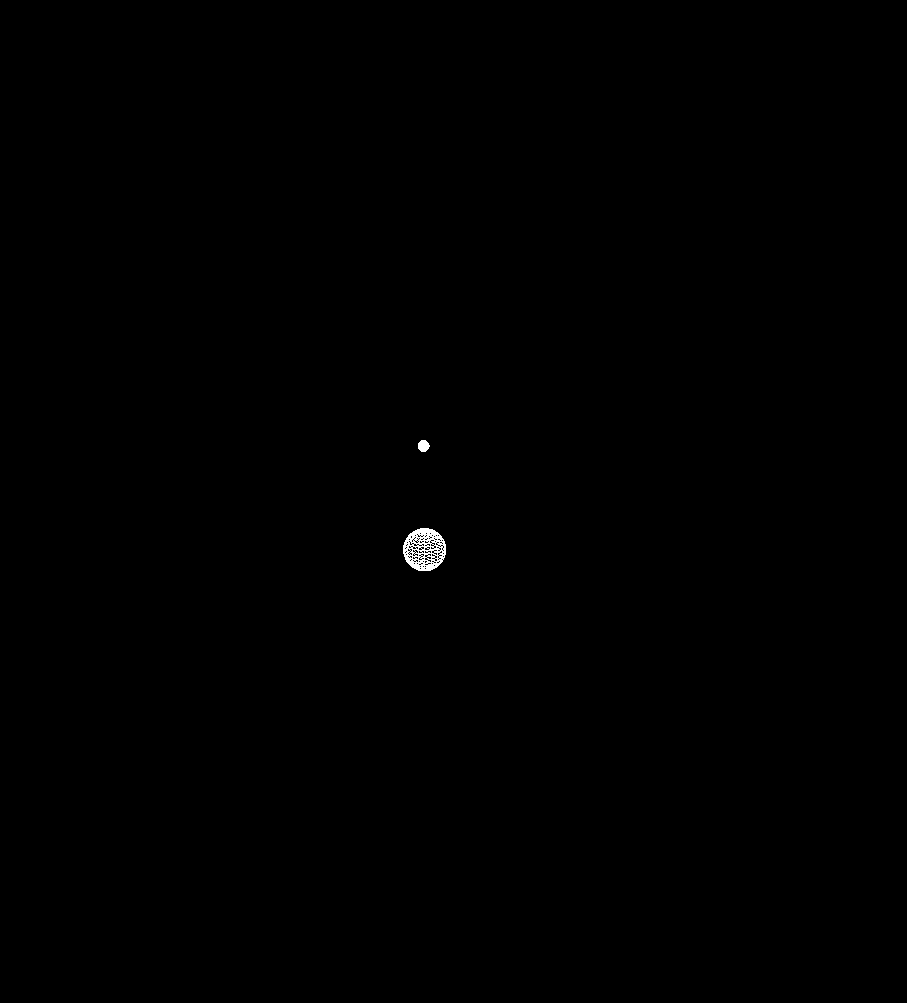
\includegraphics[width=0.9\textwidth]{solar_system_earth.png}
    \caption{Terra}
    \label{fig:sub6}
    \end{subfigure}%
    \\
    \begin{subfigure}{.5\textwidth}
    \centering
    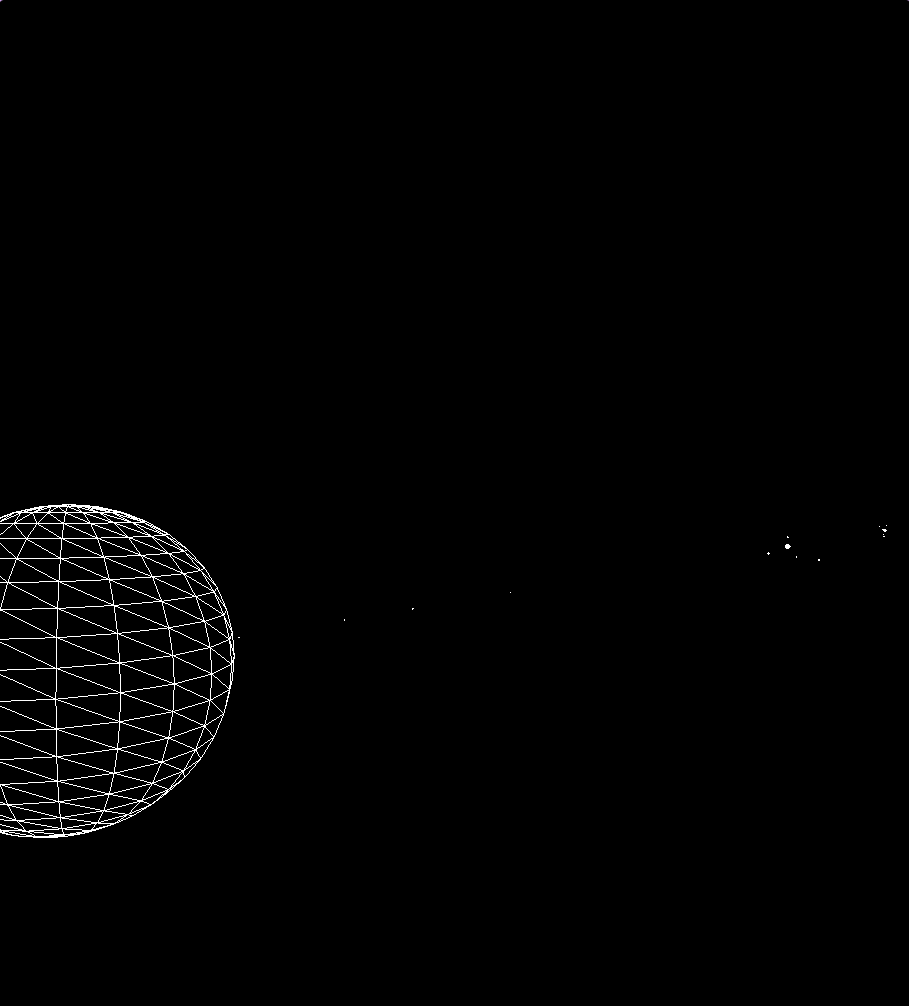
\includegraphics[width=0.9\textwidth]{solar_system_sun.png}
    \caption{Sol}
    \label{fig:sub5}
    \end{subfigure}%
    \begin{subfigure}{.5\textwidth}
    \centering
    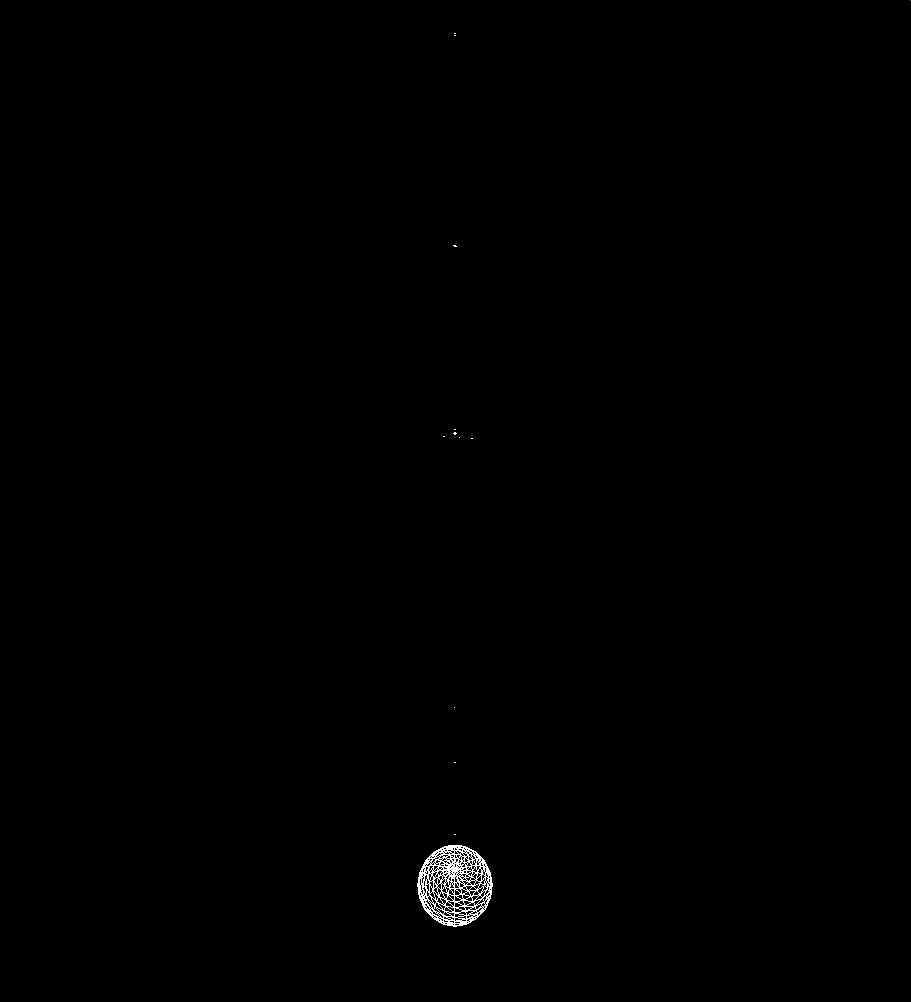
\includegraphics[width=0.9\textwidth]{solar_system_up.png}
    \caption{Sistema Solar visto de cima}
    \label{fig:sub6}
    \end{subfigure}%
    \label{fig:2}
\end{figure}

\chapter{Conclusão} \label{chap:conclusion}

Em suma, ao longo deste relatório foi implementada duas formas extras de transformação, baseadas em anteriores. Também foi implementada a possibilidade de criar primitivas gráficas a partir de superfícies de Bezier. O desenho das primitivas foi potenciado pela utilização de \textbf{VBOs}, com índices escritos nos ficheiros dos modelos para melhor optimizar este processo. Por fim, a demo foi aumentada para incluir movimentação dos astros e um cometa modelado a partir do cometa de Halley.

\end{document}

